\documentclass{jsarticle}
\usepackage[dvipdfmx]{graphicx}
\usepackage{listings,jlisting}
\usepackage{amsmath}
\usepackage{float}

\title{情報工学実験2 教育システム設計 第二回\\
        項目反応理論:1問からの能力値推定}

\author{学生番号4617043 神保光洋}
\date{\today}
\begin{document}
\maketitle

\section{要旨}
複数問についてベイズの定理、最尤推定を使用し実データを用いて能力推定する。
対数関数の活用を行う。

\section{目的}
より複雑な状況での能力推定を演習として行う。また、チャレンジ課題として、ニュートン法を用いた
能力推定についても行う。

\section{理論}
複数の問題に対する正誤判定を得た場合の能力値の推定について考える。
今、ある問題系列について正誤反応$X_j = (x_{1,j} x_{2,j},...,x_{n,j})$ が与えられたとする。
この時の能力値 $\theta$ の推定値を考えると以下のような数式を考えれば良い。

\begin{eqnarray*}
  \hat{\theta} &=& \underset{\theta}{\arg \max} P(\theta | X_j) \\
               &=& \underset{\theta}{\arg \max} P(\theta)P(X_j | \theta)
\end{eqnarray*}

ここで$P(X_j | \theta)$ はある能力値 $\theta$ の受験者が、それぞれの項目に$X_j$のように反応
する確率である。そのため、それぞれの項目への正誤が$\theta$
のみに影響され定めるとすれば、$P(X_j| \theta)$ は以下のように書ける。


\begin{eqnarray*}
  P(X_j | \theta) &=& P(x_{1,j} | \theta) \times P(x_{2,j} | \theta) \times \cdots \times P(x_{n,j} | \theta) \\
                  &=& {\prod}^{n}_{i=1} P(x_{i,j}| \theta)
\end{eqnarray*}

つまり、複数のサイコロを同時に投げた時と同様に同時確率とみなすことができる。それぞれの
項目へ能力値$\theta$だけを媒介に同時に正誤判定していると考える。これを局所独立仮定という。
すなわち、それぞれの項目が他の項目の答えやヒントになっていない状況である。

また、$P(x_{i,j}| \theta)$は正答の場合と誤答の場合両方を表すが以下のように表すことができる。

$P(x_{i,j}| \theta) = {P_i(\theta)}^{x_{i,j}} \times {(1 - P_i(\theta))}^{1 - x_{i,j}}$

したがって、考えるべき式は以下のようになる。

\begin{eqnarray*}
  \hat{\theta} &=& \underset{\theta}{\arg \max} P(\theta | X_j) \\
               &=& \underset{\theta}{\arg \max} \ln P(\theta | X_j)
\end{eqnarray*}

そのため、実装上は以下を計算すれば良い。

\begin{eqnarray*}
  \hat{\theta} &=& \underset{\theta}{\arg \max} P(\theta | X_j) \\
                && + {\Sigma}^n_{i=1}(x_{i,j} \ln (P_i(\theta)) + (1 - x_{i,j}) \ln (1 - P_i(\theta)))
\end{eqnarray*}

これを対数尤度関数と呼ぶ。

\section{課題}
\subsection{課題3-1}
課題2-3で描いた事後分布とその対数尤度関数を図示し、それぞれの最大値にどのような関係があるか示せ。

\begin{figure}[H]
  \centering
  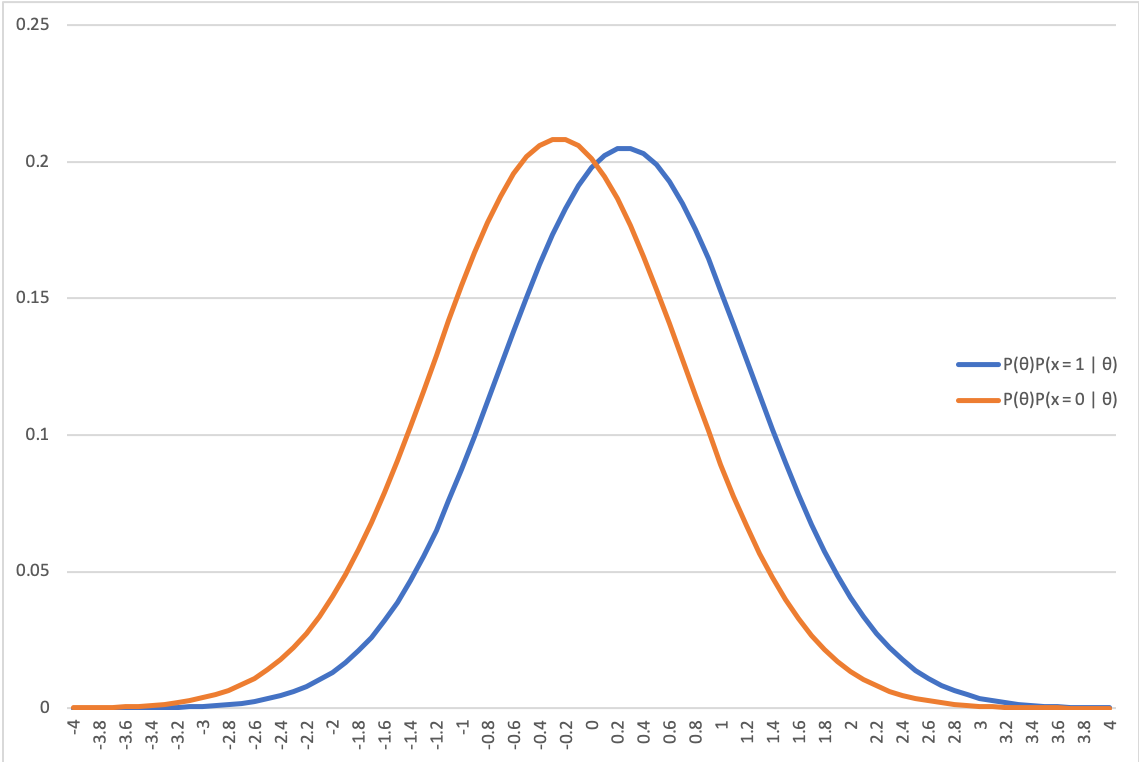
\includegraphics[width=12cm]{./key2.png}
  \caption{事後分布}
\end{figure}

\begin{figure}[H]
  \centering
  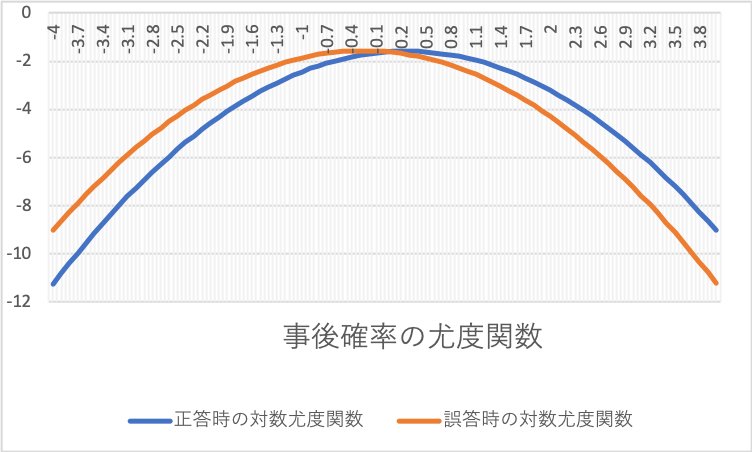
\includegraphics[width=12cm]{./ln_yuudo.png}
  \caption{対数尤度関数}
\end{figure}

グラフから最大値をとる値は同じであると示される。

\subsection{課題3-2}
表2を参考に課題1-3で解いた全ての項目の反応から自分の能力値$\theta$の対数尤度関数の概形を示せ。

\begin{figure}[H]
  \centering
  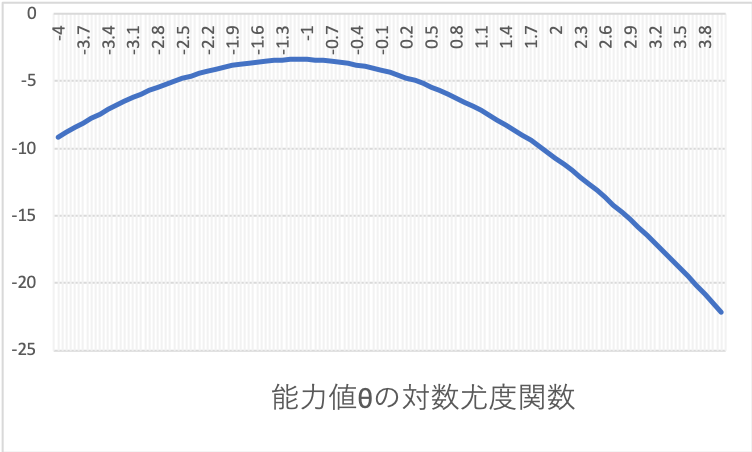
\includegraphics[width=12cm]{./all_yuudo.png}
  \caption{自分の能力値$\theta$の対数尤度関数}
\end{figure}

\subsection{課題3-3}
課題3-2で描いた対数尤度関数から能力値を推定せよ。またその時の情報量$I(\hat{\theta})$と標準誤差
$se(\hat{\theta})$を求めよ。

グラフから能力値は-1.1であると推定される
またそのとき
情報量は
$I(\hat{\theta}) = 0.303$

標準誤差は
$se(\hat{\theta}) = 1.813$

と求められる。

\section{参考文献}
\begin{thebibliography}{9}
  \bibitem{key1} 東京大学教養学部統計学教室 統計学入門 (基礎統計学Ⅰ)・東大出版会
\end{thebibliography}

\section{付録}

\end{document}
